% \documentclass[11pt, twocolumn]{article}
\documentclass[letterpaper, 10 pt, conference]{ieeeconf}
\IEEEoverridecommandlockouts
\overrideIEEEmargins


% \IEEEoverridecommandlockouts               % This command is only needed if
%                                            % you want to use the \thanks command

% \overrideIEEEmargins                     % Needed to meet printer requirements.

\usepackage[backend=biber, style=ieee]{biblatex}
\usepackage{amsmath}
\usepackage{graphicx}
\usepackage{fullpage}
\usepackage{subcaption}
\usepackage{url}
\usepackage{csquotes}
\usepackage[american]{babel}
\usepackage{comment}
% \usepackage{amsthm}

\newtheorem{theorem}{Theorem}
\newtheorem{lemma}[theorem]{Lemma}

% \DeclareMathOperator{\atantwo}{atan2}

% \DeclareMathOperator{\arctantwo}{arctan2}

%\setlength{\belowcaptionskip}{-6pt}
\setlength{\textfloatsep}{8pt}

\newcommand{\parallelsum}{\mathbin{\!/\mkern-5mu/\!}}


\DeclareMathOperator{\atantwo}{atan2}

\DeclareMathOperator{\arctantwo}{arctan2}


\addbibresource{abrv.bib}
\addbibresource{refs-chains.bib}
\addbibresource{djbref.bib}
\addbibresource{swarm.bib}
\addbibresource{peg-in-hole.bib}



\title{Finding the best insertion-based joints}
\author{Zhibin Zou \and Weifu Wang}
\date{}

\newcommand{\bo}{\mathbf o}
\newcommand{\bq}{\mathbf q}
\newcommand{\bp}{\mathbf p}
\newcommand{\bd}{\mathbf d}
\newcommand{\bn}{\mathbf n}
\newcommand{\bc}{\mathbf c}

\begin{document}
\maketitle

\begin{abstract}
In this work, we study how to find the best design for insertion-based joints, to ensure the ease of insertion subject to manufacturing errors, and the stability after insertion under external disturbances. The design analysis is built on the discretization of both the insertion process and the stability analysis. Under the assumption of a point-edge contact, we alternate the optimization of the location of contact points on the peg and the edge angles on the socket to allow minimum rotation after insertion while allowing the insertion to succeed. We find the best 2D design first, then project to 3D for the block design. The 2D design results are compared both theoretically and through simulations. 
\end{abstract}

\section{Introduction}

In this work, we present an automated design process to find the best insertion-based joint design, which we refer as {\em joineries}. Joineries have been widely used in constructions, and recently, automated assembly using such joineries has been studied~\cite{Zhang2018-interlocking}. The joineries, together with the blocks which the joineries are attached to, relying on their geometries to interlocks the blocks during assembly and secure the assembled structure. 

We measure the quality of the design from two perspectives: the chance of success for insertion, and the stability of the peg in the socket after insertion. The analysis for stability has been studied before, though mostly as an analysis tool, such as the method presented in~\cite{Lensgraf20}. This work proposes to optimize the design for both the execution (insertion) and the structure stability. 

Our analyze builds upon the assumption of point-edge (surface) contact between the peg and the socket, which is a common assumption in the analysis of caging. In previous work, when we designed for surface contacts between pegs and sockets, in practice, the manufacturing error often destroyed the assumption, thus lead to unpredictable behaviors of the joints both during and after the insertion. The main cause of the unpredictable behaviors is the unknown actual contact locations between the peg and the socket. Under the assumption of the point-surface contact, even when error can exist, as long as the error is upper bounded and smaller than the design clearance on the peg between the designed contacts and the body of the peg, a point-surface contact design can always result in known contact locations between peg and the socket. 

The design process presented in this work is a numerical process relying on sequences of optimizations. Due to the numerical instability, even under the assumption of linear edges and surfaces, the global optimal solution can be difficult to find. The detail of the design process is presented in Section~\ref{sec:design}. We analyze the insertion process and the stability after insertion separately, and using each process to find the {\em gradient} information of how design changes can affect the insertion and stability respectively. Using the derived information, improved design will be found and analyzed again until limited improvements can be made. 

The design process also starts from the 2D plane, finding the {\em best} 2D design for a pair of peg and socket, and can then be projected to 3D to build actual blocks. This work focus on the design process in 2D, and the different projection approaches will be studied and analyzed in the future work. We conducted simulations for insertion in bullet physics engine~\cite{coumans2019}, validating our analysis and design output. 



\section{Related work}

Assembly with joineries has a long history in construction, such as the dovetail and mortise and tenon are used in carpentry around the world. Most such approaches were engineered and carried out entirely by humans. The major difference between the joinery based assembly and the brick-cement based assembly is the lack of {\em glues} and bonding materials~\cite{zwerger2012wood}, which make the assembly process reversible. Recently, it has been hypothesized that the backbones of theropod dinosaurs interlocked to provide support for the extremely large body mass~\cite{woodruff2016}.

Reconfigurable assembly relying on geometric constraints has been well studied~\cite{song2012recursive, song2017reconfigurable, songcofifab, fu2015computational, Wang-2018-DESIA}. Different interlocking designs has been proposed in the past~\cite{Yao:2017:IDS:3068851.3054740}. 

Autonomous assembly with robots has also been explored before. Andres {\em et al.} created ROCCO to grasp and lay-down blocks for assembly~\cite{andres1994first}, and the similar system was later adapted by Balaguer {\em et al.}~\cite{balaguer1996site}. More systems have been developed recently, such as the system developed by Helm {\em et al.}~\cite{helm2012mobile} and by Giftthaler {\em et al.}~\cite{giftthaler2017mobile}. More novel construction approaches with drones and 3D printing technologies were also explored recently~\cite{willmann2012aerial, augugliaro2014flight, lindsey2011construction, augugliaro2013building, keating2017toward, winsun3dprint}. 

To allow the automation of the joinery-based assembly, there are some compromises one need to make. The joinery design needs to be less complicated for the ease of manufacturing and mass production. Also, the mechanism proposed by the joineries should be simple enough so that even with little adaptability, the robot devices can successfully supply the motions needed for the connection of joineries. Naturally, the joinery-based assembly extends from the idea of modular robots and assembly~\cite{rus2001crystalline, white2005three, romanishin2013m, daudelin2017integrated}. Recently, Schweikardt {\em et al.}~\cite{schweikardt2006roblocks} proposed an educational kit for robotic construction, inspired by LEGO. 

The simplest joint design is insertion-based, where the assembly process is just repeatedly apply translations to blocks while relying on the geometries of the blocks to secure the constructed structure. The classic peg-in-hole problem models this insertion strategy, which was studied by Lozano-Perez {\em et al.}~\cite{Lozano-Perez1984}. Building on the back-chaining approach, many similar systems were developed to study the insertion-based assembly approach~\cite{Mason86, Bruyninckx95, ZhangZOH04}. However, most study focus on the strategy for the insertion rather than the design of the joints. 

The automated design process presented in this work relies on numerical optimization, and a discretization of change in contacts during motion. In 2002, Balkcom {\em et al.} analyzed the possible motions of rigid objects under multiple contacts and given forces~\cite{Balkcom2002c}. In Moll's thesis~\cite{Moll2002}, a similar discretization approach was adapted to study the contacts between hands and objects. In this work, we also assume the linear edges in the socket design, thus using an linear approximation of more complex shapes. Linear approximation can greatly simplify the optimization process and find good results locally. For example, Berenson used linear approximation to study the effect of force applied to flexible objects~\cite{Berenson2013-deformable}. 

In this work, we adapted the assumption of point-surface contact, making the problem an extension of the caging problem~\cite{RimonBlack96, Rodriguez2010}. However, as the caging studies instances of contacts between fingers and objects, the design process introduced in this work also considers the changes and consequences of different contacts and forces. 


\section{Joint design process}
\label{sec:design}


In this section, we present the details of the design process, which are derived under the assumption of the existence of error, either from manufacturing or execution. For simplicity of analysis, the manufacturing error is assumed to be uniform, and was only applied to the socket while the peg is {\em perfect}. Both the peg and the socket are part of a block, which is of limited size, making the size of the peg and the socket limited with respect to the block. We also assume that the friction coefficient is a fixed given value. 

The design process for insertion and the stability after insertion are analyzed separately. During insertion, the main goal is for the peg to be fully inserted into the socket, regardless of the initial configuration or the intermediate stages the insertion has to go through. The initial insertion configuration of the peg is assumed to be within a bounded error of the perfect insertion location and orientation, simulating the sensing error and grasping error during assembly. The success of transition between different stages is the key to reaching the desired inserted configuration, which we refer as a {\em sink}. The analysis of the insertion stage focus on ensuring the success of these transitions. 

After the insertion, the peg may move within the socket under external disturbance, if the manufacturing error exists. As the relative translation of the peg within the socket is unavoidable, the main goal for the peg stability is to achieve the minimum possible rotation within the socket. A design change that reduces such rotation is considered an improvement, and finding such changes is the goal for the stability analysis. 

As the design of the joint consists of two parts, the peg and the socket, we will consider the change of one component of the joint only for each process. On the peg, we study the effect of moving the desired contact locations along the contact edge of the socket, mostly in terms of stability of the peg after insertion. On the socket, we consider the effect of the change of the angles of different edges. The change of the edge angle, however, may affect both the stability and the success of insertion. In the proposed design process, we will first ensure the success of insertion before optimizing for the stability when it comes to socket design. 


\subsection{Insertion process analysis}

% During the insertion, the peg may contact the socket along different edges at different locations. Maintaining the contacts at different edges require different set of constraints if expressed as constraints in an optimization process. To ensure the success of insertion, there are different sets of constraints one needs to maintain, depending on the {\em stage} of insertion. This makes the straight optimization of joint design difficult to model. 

Insertion process may change how peg and socket contact each other as the insertion progresses, thus describing the contacting constraints can be difficult. On the other hand, the different sets of constraints can be considered separately, if we discretize the insertion process. We define {\em Mode of Contacts} as a collection of point-edge pairs that are in contact, and to each point-edge pair that is in contact as a {\em Contact Pair}, denoted as $CP(i, j) = \{p_i, e_j\}$. We use $p_i$ to denote the $i$th point on the peg following a counter-clockwise order, and $e_j$ to denote the $j$th edge on the socket in the counter-clockwise order. We also denote the Mode of Contact as $MoC(k) = \{CP(a, b), CP(c, d), \ldots\}$. Then, the entire insertion process can be described as a directed graph when the insertion is guided by a known force. 

In this paper, we only consider the Contact-Pair as the pair containing a point on a peg and an edge on the socket. For simplicity, the points on the peg can be joined by different designs (curves) to avoid any contact between the socket edges other than the bounded number of designed contact points. In addition, a point on the peg contacting two adjacent edges on the socket, i.e., a point-point contact, can be viewed as two contact pairs. Therefore, the Contact-Pair defined above is the fundamental unit for analyzing the Mode of Contact in the peg-socket relation. 

We will first find the set of all valid Mode of Contacts (MoCs). In order for a Mode of Contact to be valid, each containing Contact Pair need to be valid for the given peg and socket, and a valid configuration must exist to allow the set of Contact Pairs to co-exist. We adapted a bottom up approach to find the valid MoCs: identifying all valid Contact Pairs (CPs), and find all combinations of CPs to form potential valid MoCs; for each of the candidate valid MoC, we test if there exist a valid configuration allowing the set of CPs co-exist. 

The MoCs alone cannot fully describe the insertion process, as the insertion process also involves the transition between different modes. To find out whether a transition between two Mode of Contact under a given force is possible, we can find the acceleration direction under the insertion force, and the location of the different CPs between the two modes. If the acceleration / moving direction can lead to the contact or the removal of the corresponding point-edge pairs, then the transition is valid, otherwise not. 

There is a huge number of possible transitions among all valid MoCs. For simplicity, we can view a potential transition between arbitrary two modes as a sequence of transitions between two {\em adjacent modes}. Given $MoC(i)$ and $MoC(j)$, if the difference between the two MoCs is $d$ Contact Pairs $CP_k(a, b), 1\leq k\leq d$, then we refer these two MoCs as {\em $d$-neighbors}. We can show that arbitrary {\em valid} transition between two MoCs during insertion can be decomposed to either a sequence of transitions between $1$-neighbor MoCs, or a special transition between $k$-neighbors where $k$ can be uniquely computed for given peg and socket, and there can only exist a bounded number of special transitions. In addition, add a special MoC with no contact pairs. 

\begin{lemma}
Given a peg as a sequence of $n$ points $p_i$ where no two points are designed to contact the same edge on the socket, a socket of a sequence of $m$ edges $e_i = (p^e_i, p^e_{i+1})$ with uniform manufacturing error $\epsilon$, a insertion force along the orientation of the peg, and a distance function $d(\cdot)$, if $d(p_i, p_j) \neq d(p^e_s, p^e_t) \forall i, j\in\{1, 2, \ldots, n\}, s, t\in\{1, 2, \ldots, m+1\}$, then if a transfer from $MoC(a)$ to $MoC(b)$ can happen, there always exist a sequence of transitions from $MoC(k_i), k_1 = a, k_n = b$ where the difference between $MoC(k_i)$ and $MoC(k_{i+1})$ is no more than a single Contact Pair. 
\end{lemma}

\begin{proof}
Let there be two Mode of Contacts $MoC(a)$ and $MoC(b)$ where a transition from $MoC(a)$ to $MoC(b)$ is possible, and the two modes differ by more than a single contact pair. Let there do not exist $MoC(c)$ where both $MoC(a)$ to $MoC(c)$ and $MoC(c)$ to $MoC(b)$ are possible. 

Without loss of generality, let $|MoC(b)| > |MoC(a)|$. and let $CP(i, s)$ and $CP(j, t)$ be the two contact pairs that cannot be introduced independently. There are two cases, 1) the peg can rotation even for the same contact location along the edge; 2), the orientation of the peg in $MoC(a)$ depends only on the contact location for the contact pairs, i.e. for the same contact location along the edges, no rotation is permitted. 

In the case 1, the only scenario is that there is only one contact pair in $MoC(a)$. In this case, as the orientation of the peg can change even when the contact pair does not change relative location, there does not exist design where $CP(i, s)$ and $CP(j, t)$ must make contact together unless some $d(p_i, p_j) = d(p^e_s, p^e_t)$, as any change of the orientation of the peg will change the relative distance between the pending contact pairs, preventing the simultaneous contact. 

In the case 2, as the socket has error, if the insertion angle is perfect aligned with the depth of the socket, no such $CP(i, s)$ and $CP(j, t)$ exist, as no two points are designed to contact the same edge, thus no simultaneous contacts. If the insertion angle is off by $\delta$, then unless the socket has non-uniform error, the rotation of the peg cannot permit multiple contact pairs to happen at the same time while they can also make contact when fully inserted into the no-error socket. 
\end{proof}

We therefore can define a directed graph $G = (V, E)$, where $V$ is the set of valid MoCs, and $E$ are the valid transitions between neighbor modes or among special modes. We refer this graph as the Contact Mode Transition (CMT) graph. Then, for each vertex on the graph, the set of constraints describing the relation between peg and socket is of fixed number. 

To simulate the sensing error during automated assembly, we introduce $\Delta x$ and $\Delta\phi$ during insertion, denoting the maximal offset along $x$ axis and the maximal rotation allowed at the beginning of the insertion. The values are bounded by the precision of the sensing technology. We define the beginning of the insertion as the moment the peg and the socket first make contact. Under such initial error, we would like the designed peg to still be able to be inserted into the socket. 

One of the necessary condition for the success of insertion is the peg not contacting any edge outside the socket, which we refer to as the {\em capture} of the peg. In the remaining section of paper, for simplicity of illustration, we connected contact points on the peg with straight edges in the figures, but the actual design may require these connection to be curved to avoid undesigned contacts. Figure~\ref{fig:capture} shows an example of the peg not captured by the socket (left); and by rotating the top-left edge of the socket, the peg can be captured with the same $\Delta x$ and $\Delta\phi$ (right). If a peg can be captured by the socket, we can derive its CMT graph. 

\begin{figure}[t]
\begin{center}
\begin{subfigure}[t]{0.23\textwidth}
\begin{center}
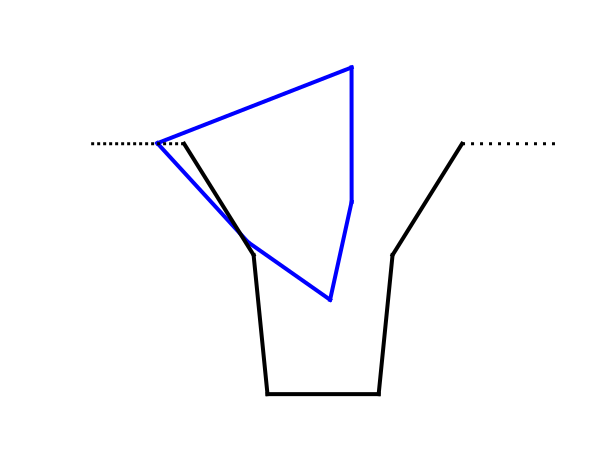
\includegraphics[height=1.2in]{figures/not_capture.png}
\end{center}
% \caption{The peg is not captured by the socket. }
% \label{fig:not_capture}
\end{subfigure}
\begin{subfigure}[t]{0.23\textwidth}
\begin{center}
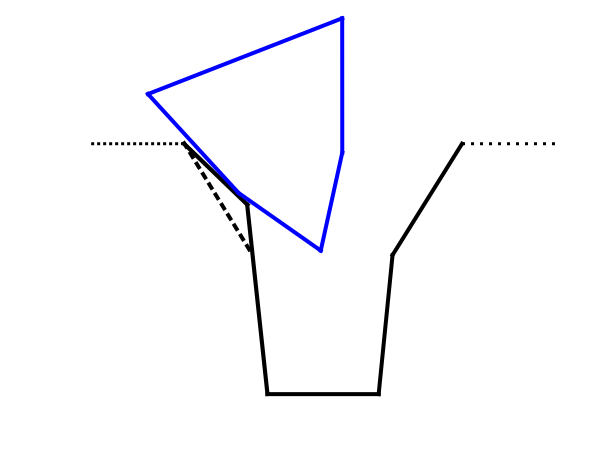
\includegraphics[height=1.2in]{figures/captured.png}
\end{center}
% \caption{The peg is captured by the socket.}
% \label{fig:captured}
\end{subfigure}
\caption{An example of peg not captured by the socket, and how the socket can be changed to guarantee the capture. }
\label{fig:capture}
\end{center}
\end{figure}


Define a {\em sink} on the CMT graph as a vertex that either has only in coming edges, or has bi-directional edges with another {\em sink}. A insertion process can be considered successful only if the CMT graph has sinks. The inverse statement is not true, as some sinks may not be desired. For example, a CMT graph for a five-edge socket and a five-point peg is shown in Figure~\ref{fig:insertion_graph}, four sinks are identified, and are shown in Figure~\ref{fig:5_5_sink}. The sinks shown in Figure~\ref{fig:5_5_sink2} and~\ref{fig:5_5_sink3} are not desired, as the peg is not fully inserted and by definition the peg cannot get out of the MoC under the insertion force. 

If no manufacturing error is present, there should exist one and only one sink, the mode with the most contact pairs. When the manufacturing error is present, the largest number of contact pairs may not be achieved. A sink is {\em undesirable} if there exist other sinks with more contact pairs. What is more, isolated sinks are not desired when error exists. 


\begin{figure}
\begin{center}
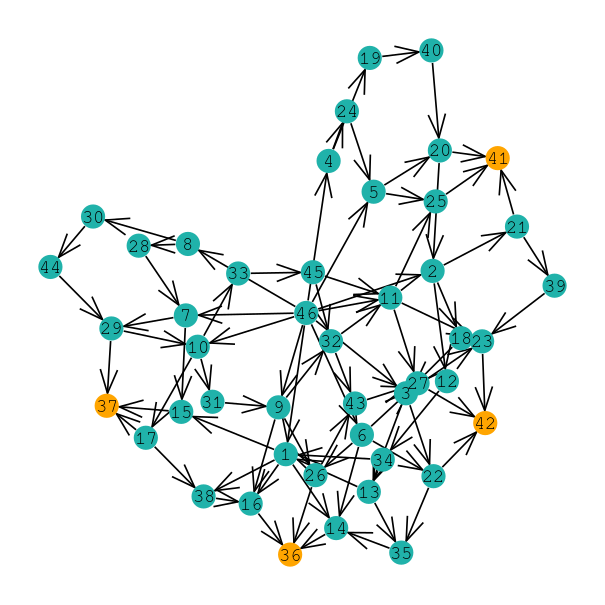
\includegraphics[width=3in]{figures/insertion_graph.png}
\end{center}
\caption{The insertion graph of a five-point and five-edge peg-socket joint. }
\label{fig:insertion_graph}
\end{figure}


\begin{figure*}
\begin{center}
\begin{subfigure}[t]{0.24\textwidth}
\begin{center}
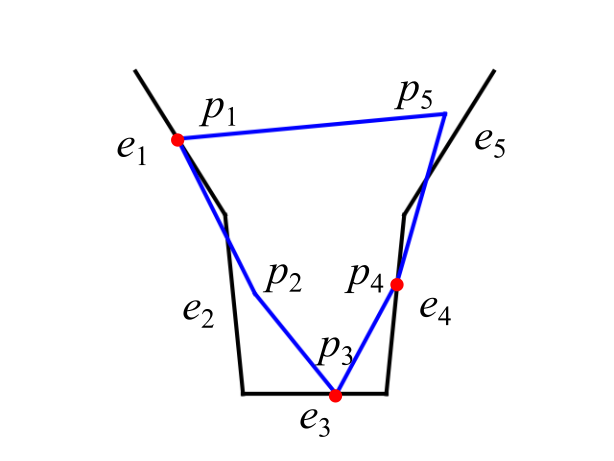
\includegraphics[height=1.3in]{figures/5_5_sink1.png}
\end{center}
\caption{Sink 1. $MoC(36)$ with $CP(1, 1)$, $CP(3, 3)$ and $CP(4, 4)$.}
\label{fig:5_5_sink1}
\end{subfigure}
\begin{subfigure}[t]{0.24\textwidth}
\begin{center}
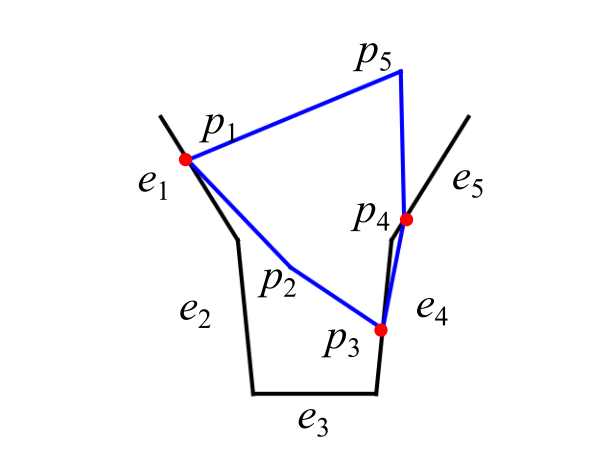
\includegraphics[height=1.3in]{figures/5_5_sink2.png}
\end{center}
\caption{Sink 2. $MoC(36)$ with $CP(1, 1)$, $CP(3, 4)$ and $CP(4, 5)$. }
\label{fig:5_5_sink2}
\end{subfigure}
\begin{subfigure}[t]{0.24\textwidth}
\begin{center}
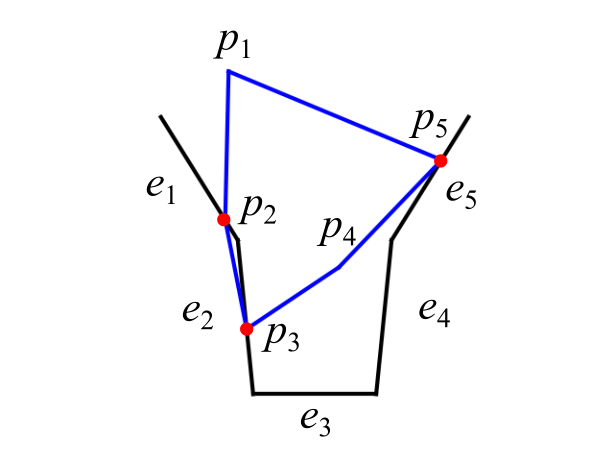
\includegraphics[height=1.3in]{figures/5_5_sink3.png}
\end{center}
\caption{Sink 3. $MoC(41)$ with $CP(2, 1)$, $CP(3, 2)$ and $CP(5, 5)$. }
\label{fig:5_5_sink3}
\end{subfigure}
\begin{subfigure}[t]{0.24\textwidth}
\begin{center}
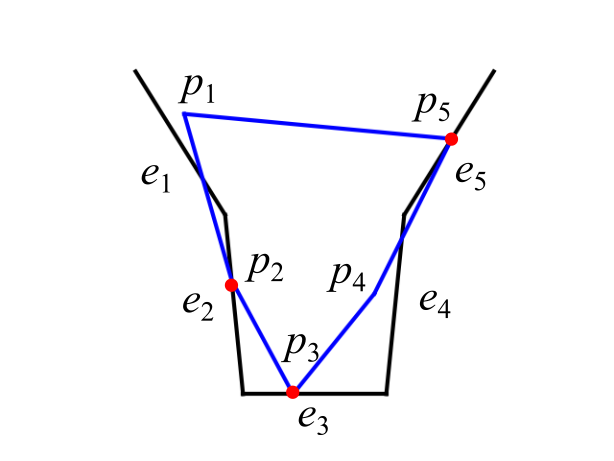
\includegraphics[height=1.3in]{figures/5_5_sink4.png}
\end{center}
\caption{Sink 4. $MoC(42)$ with $CP(2, 2)$, $CP(3, 3)$ and $CP(5, 5)$.  }
\label{fig:5_5_sink4}
\end{subfigure}
\end{center}
\caption{Sinks of an insertion CMT graph for joint with five-point peg and five-edge socket. }
\label{fig:5_5_sink}
\end{figure*}

\subsection{Stability after insertion}

Another important criteria for a good peg-socket design is how stable the peg will be in the socket after insertion, under external disturbances and subject to manufacturing error. Under the assumption of an uniform error on the socket, translation of the peg inside the socket after insertion is unavoidable regardless of the design. As the designed joints will be part of blocks with fixed size, we further assume the socket and the peg have bounded maximum width and depth. 

% The question then becomes, how will the different designs of peg and socket reduce possible rotations after insertion? 

% Intuitively, given the uniform error $\epsilon$ between the peg and the socket, the longer the peg is, the less rotation is possible after insertion. However, as the peg and the socket are both part of a block, which has bounded size, we have to assume the maximum depth of the socket is bounded. 

We again discretize the possible motions of the peg in the socket after insertion based on different Mode of Contacts (MoCs). The key observation is that, there exist a partial order of all the valid MoCs, based on the possible rotations of the peg. For example, consider the two Modes of Contact shown in Figure~\ref{fig:5_5_sink1} and~\ref{fig:5_5_sink2}, the MoC shown in Figure~\ref{fig:5_5_sink2} will always have a larger rotation compared to the MoC shown in Figure~\ref{fig:5_5_sink1}. Based on the derived partial order, we therefore only need to analyze the MoCs with the highest order, i.e. the largest possible rotation. In addition, we do not want to consider the scenarios where the peg has moved away from the socket, thus we will add a {\em virtual cap} near the entrance of the socket. 

\begin{figure}[t]
\begin{center}
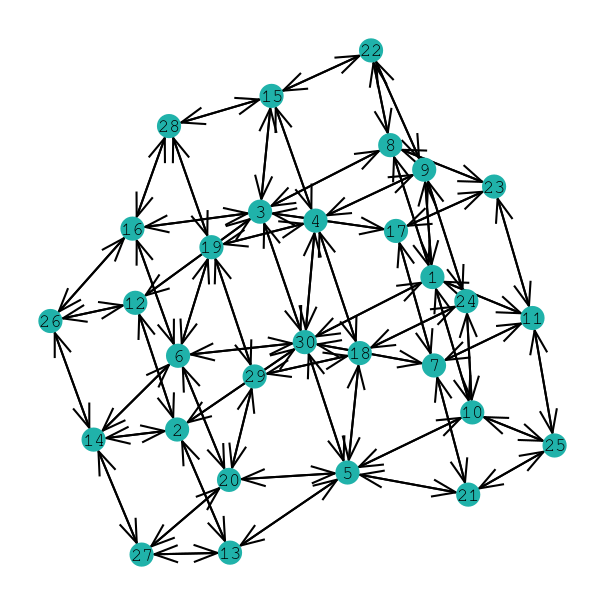
\includegraphics[width=3in]{figures/rocking_graph.png}
\end{center}
\caption{The CMT graph of the peg in socket. }
\label{fig:rocking_graph}
\end{figure}

Let us define a contact point on the peg as a function of $s$, the length along a given socket edge. Then, the design of the peg becomes a collection of pairs, $(i, s)$, where $i$ denotes the designed contacting edge for the given contact point, and $s$ is the distance along the edge following the counter-clockwise direction. This definition is only valid when no error is introduced, i.e. the design for the perfect peg and socket. 

Based on the previously derived partial order, we analyze the MoCs with the highest order, and study how does the change of $s$ can affect the rotation angle of the peg inside the socket after insertion. Then, we can effectively find a direction ({\em gradient}) of contact-point (on the peg) motion that will reduce the possible rotation. Paired with the socket-edge rotation direction that can preserve (or break) the insertion transition, we can derive the following design procedure to find the {\em best} design for the joint. 

\subsection{Design procedure}

Combining the analysis for the peg and the socket design, we present the following design procedure. 

\begin{enumerate}
% \vspace{-1em}
\item Input: an initial (arbitrary) design of $m$ edges (socket) and $n$ contact points (peg); friction coefficient $\mu$, and a force magnitude $|F|$; 
% \vspace{-1em}
\item Find all possible CPs and MoCs for insertion, generate the CMT graph for insertion ($G_I$); 
% \vspace{-1em}
\item Identify sinks, if undesired sinks exist, find edges moving directions that will remove them as sink, and change the design, until no undesired sink exist on the CMT graph; 
% \vspace{-1em}
\item For each transition, identify the direction of socket edge rotation direction that will break the transition; 
% \vspace{-1em}
\item Generate the CMT graph for stability $G_S$, generate the partial order for nodes; 
% \vspace{-1em}
\item For each of the nodes with the highest order, find the contact-point gradient for reducing rotation;
% \vspace{-1em} 
\item While $G_I$ remains the same and the rotation angle reduction $\Delta\phi$ is larger than $\delta$, the change of the edge angle or the change in $s$, iteratively move the points and rotate the edges to reduce the possible rotation after insertion; label the best design as $D$; 
% \vspace{-1em}
\item If the $G_I$ is changed, compute the new insertion CMT graph $G'_I$, see if the new graph contains undesired sinks, if no, repeat the process for $G'_I$ starting from step 4; compare the design to $D$, and output the best design; 
% \vspace{-1em}
\end{enumerate}

Using the procedure described above, with $m = 5$ and $n=5$, we can find the following design show in Figure~\ref{fig:best_5_5_joint}. The blue shape is the initial input, while the red shape is the peg design output by the procedure above. In the process, we maintained an uniform error of $\epsilon$ on the socket. 

The best design for the joint overall may not share the same $m$ and $n$ input by the user. Therefore, the procedure above should be put inside a loop that test different $m$ and $n$. However, we do not need to test $m$ and $n$ as two independent variables, as $n$ cannot be too different from $m$. If $n - m > 0$, then, there exist two or more contact points on the peg that contacts along the same edge. The co-linear contact points are redundant as one of the contact point will provide no constraint when rotated, leaving some contact points with no effect at all. Therefore, we only need to consider the case where $n - m \le 0$. Under the linear socket edge assumption in this work, we only need to consider $m$ up to 6. In the future work, we will use more edges to simulate curved socket edges, and compare to the linear socket edge designs to further validate the linear assumption. 

% Also, as six contacts are sufficient to immobilize arbitrary planar object, we only need to test $m$ up to $6$, and no less than $3$. Therefore, the complete design procedure will be the above presented procedure nested inside a loop over possible $m$ and $n$. 


\begin{figure}[t]
\begin{center}
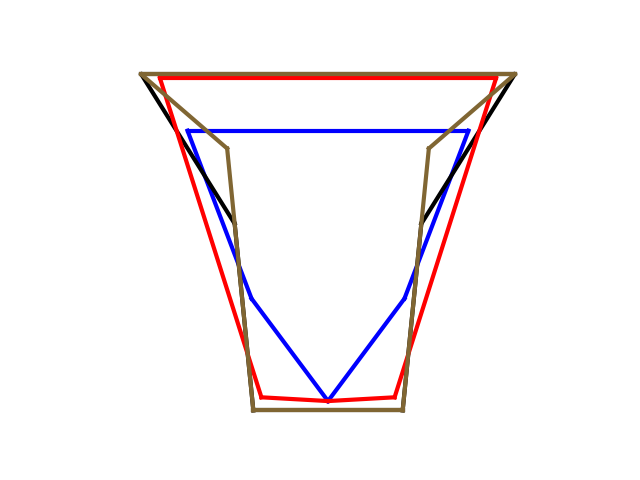
\includegraphics[width=2.3in]{figures/best_5-5_joint.png}
\end{center}
\caption{Optimized peg-socket joint design (red and brown) and given peg-socket joint (blue and black) with five peg points and five socket edge. }
\label{fig:best_5_5_joint}
\end{figure}

When the number of edges in the socket exceeds four, the shape of the socket can be either convex or concave. Under the assumption of the point-edge contact, where the points are provided by the peg and edges by socket, it can be shown that a convex shaped socket of the same number of edges would permit larger rotation after insertion for the same given $\Delta x$ and $\Delta\phi$, the initial insertion error. 

Given a $\Delta x$ and $\Delta\phi$, if when the peg makes the first contact with the socket, there exist a point $p_i$ on the peg that projects outside the socket along the $x$-axis, the further insertion will lead $p_i$ to contact some edge outside the socket. Therefore, the point $p_i$ needs to be moved further inside the along the $x$-axis. Such motion will allow larger rotation after insertion, making the peg less stable inside the socket. However, if the socket is of a concave shape, by carefully arranging the angles of edges of the socket, even when $p_i$ projects outside the socket along $x$-axis during the initial contact, $p_i$ may not contact any edge outside the socket. Such design would allow much smaller rotation after insertion. The case with convex shaped socket can be verified by computing the signed distance between points and edges of the socket, and during the motion, the signed distance will be negative when it suppose to make contact with the edges of the socket, thus create collision if $p_i$ initially projects outside the socket along $x$ axis. This has also been verified by the design process, thus all designs presented are based on sockets with concave shapes. 

In Table~\ref{tab:table1}, we compared the maximum possible rotation, i.e. stability after insertion, before and after optimization for different $m$ and $n$ combinations. The optimization process suggests that a socket with $6$ edges along with a peg with $5$ designed contact points presents the most stability after insertion, while all the optimized designs can secure the success of insertion. 

% We find the difference of the possible rotation before and after the optimization for the design, and see a big improvement for the possible rotation, in radian. As shown in Table~\ref{tab:table1}, the stability of both joints has been increased after optimizing. However, the difference of stability between the two optimized joints are very small. 

% \begin{table}[h!]
%   \begin{center}
%     \caption{Possible rotations for the joints with $m=5$.}
%     \label{tab:table1}
%     \begin{tabular}{|c | c | c | c|}
%     \hline
%       \textbf{$n-m$ } & \textbf{Max rotation} & \textbf{Max rotation} & \textbf{Max rotation}\\
%       \hline
%       4-5 joint & 0.176369 & 0.036591 & 0.036536\\
%       \hline
%       5-5 joint & 0.187765 & 0.039709 & 0.039709\\
%       \hline
%       5-6 joint & 0.194419 & 0.035660 & 0.026283\\
%       \hline
%      6-6 joint & 0.194419 & 0.040338 & 0.040150\\
%       \hline
%     \end{tabular}
%   \end{center}
% \end{table}

\begin{table}[h!]
  \begin{center}
    \caption{Stability after insertion measured by the max possible rotation angle, before and after the optimization for design.}
    \label{tab:table1}
    \begin{tabular}{|c | c | c|}
    \hline
      \textbf{$n-m$ } & \textbf{Initial input design} & \textbf{Optimized design}\\
      \hline
      4-5 joint & 0.176369 & 0.036536\\
      \hline
      5-5 joint & 0.187765 & 0.039709\\
      \hline
      5-6 joint & 0.194419 & 0.026283\\
      \hline
     6-6 joint & 0.194419 & 0.040150\\
      \hline
    \end{tabular}
  \end{center}
\end{table}



\begin{figure}
\begin{center}
\begin{subfigure}[t]{0.23\textwidth}
\begin{center}
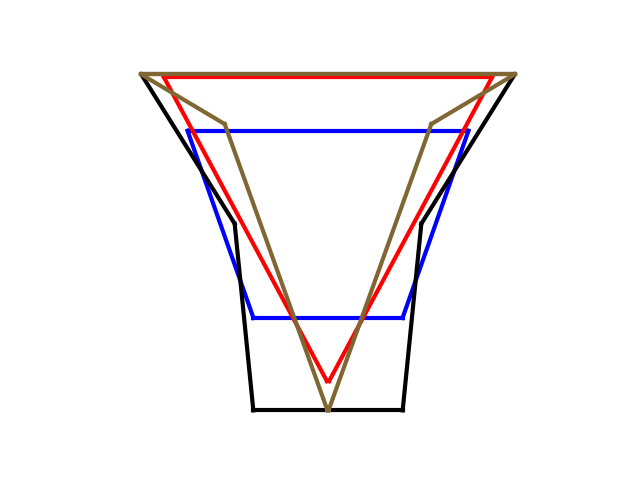
\includegraphics[height=1.2in]{figures/best_4-5_joint.png}
\end{center}
\caption{Case for $m = 5, n = 4$. }
\label{fig:best_4-5_joint}
\end{subfigure}
\begin{subfigure}[t]{0.23\textwidth}
\begin{center}
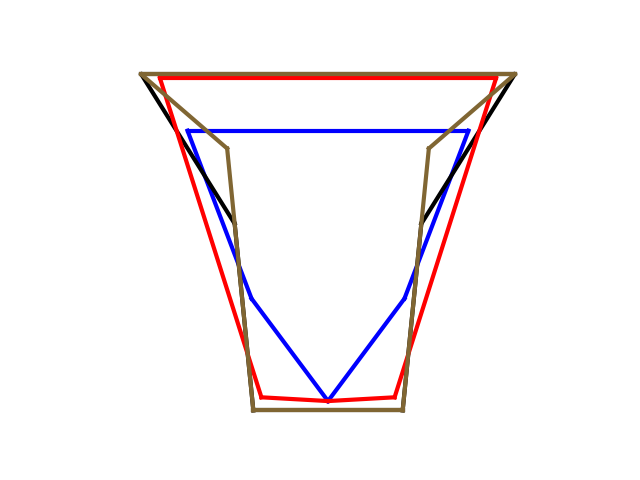
\includegraphics[height=1.2in]{figures/best_5-5_joint.png}
\end{center}
\caption{Case for $m = 5, n = 5$. }
\label{fig:best_5-5_joint}
\end{subfigure}
\begin{subfigure}[t]{0.23\textwidth}
\begin{center}
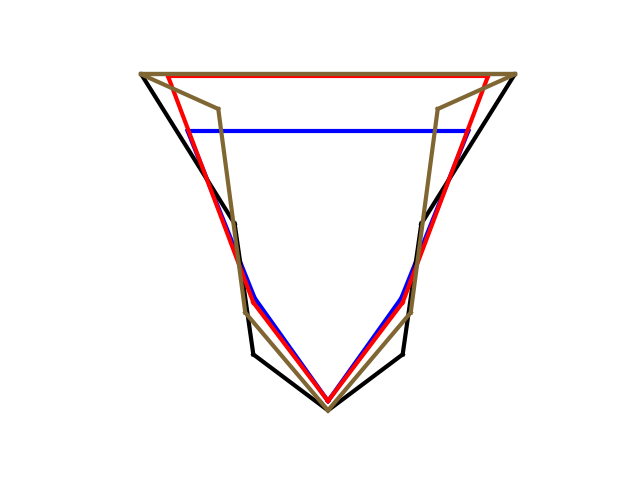
\includegraphics[height=1.2in]{figures/best_5-6_joint.png}
\end{center}
\caption{Case for $m = 6, n = 5$. }
\label{fig:best_5-6_joint}
\end{subfigure}
\begin{subfigure}[t]{0.23\textwidth}
\begin{center}
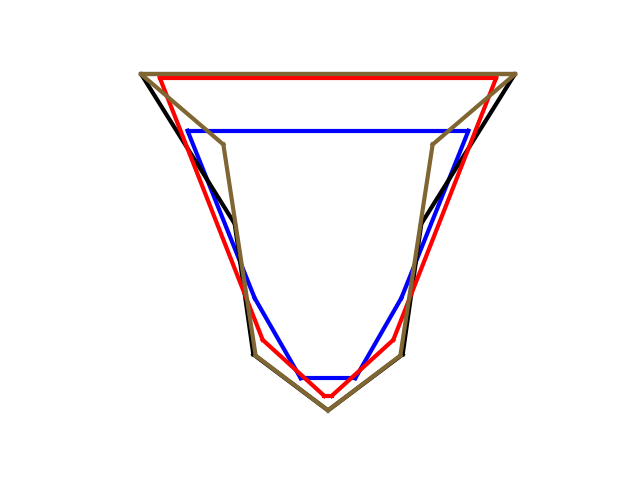
\includegraphics[height=1.2in]{figures/best_6-6_joint.png}
\end{center}
\caption{Case for $m = 6, n = 6$.  }
\label{fig:best_6-6_joint}
\end{subfigure}
\caption{The initial design (blue and black) and optimized design  (red and brown) for joints with different $m$ and $n$. }
\label{fig:best_joint}
\end{center}
\end{figure}

\subsection{Simulation in physics engine}



\begin{figure}[t]
\begin{center}
\begin{subfigure}[t]{0.23\textwidth}
\begin{center}
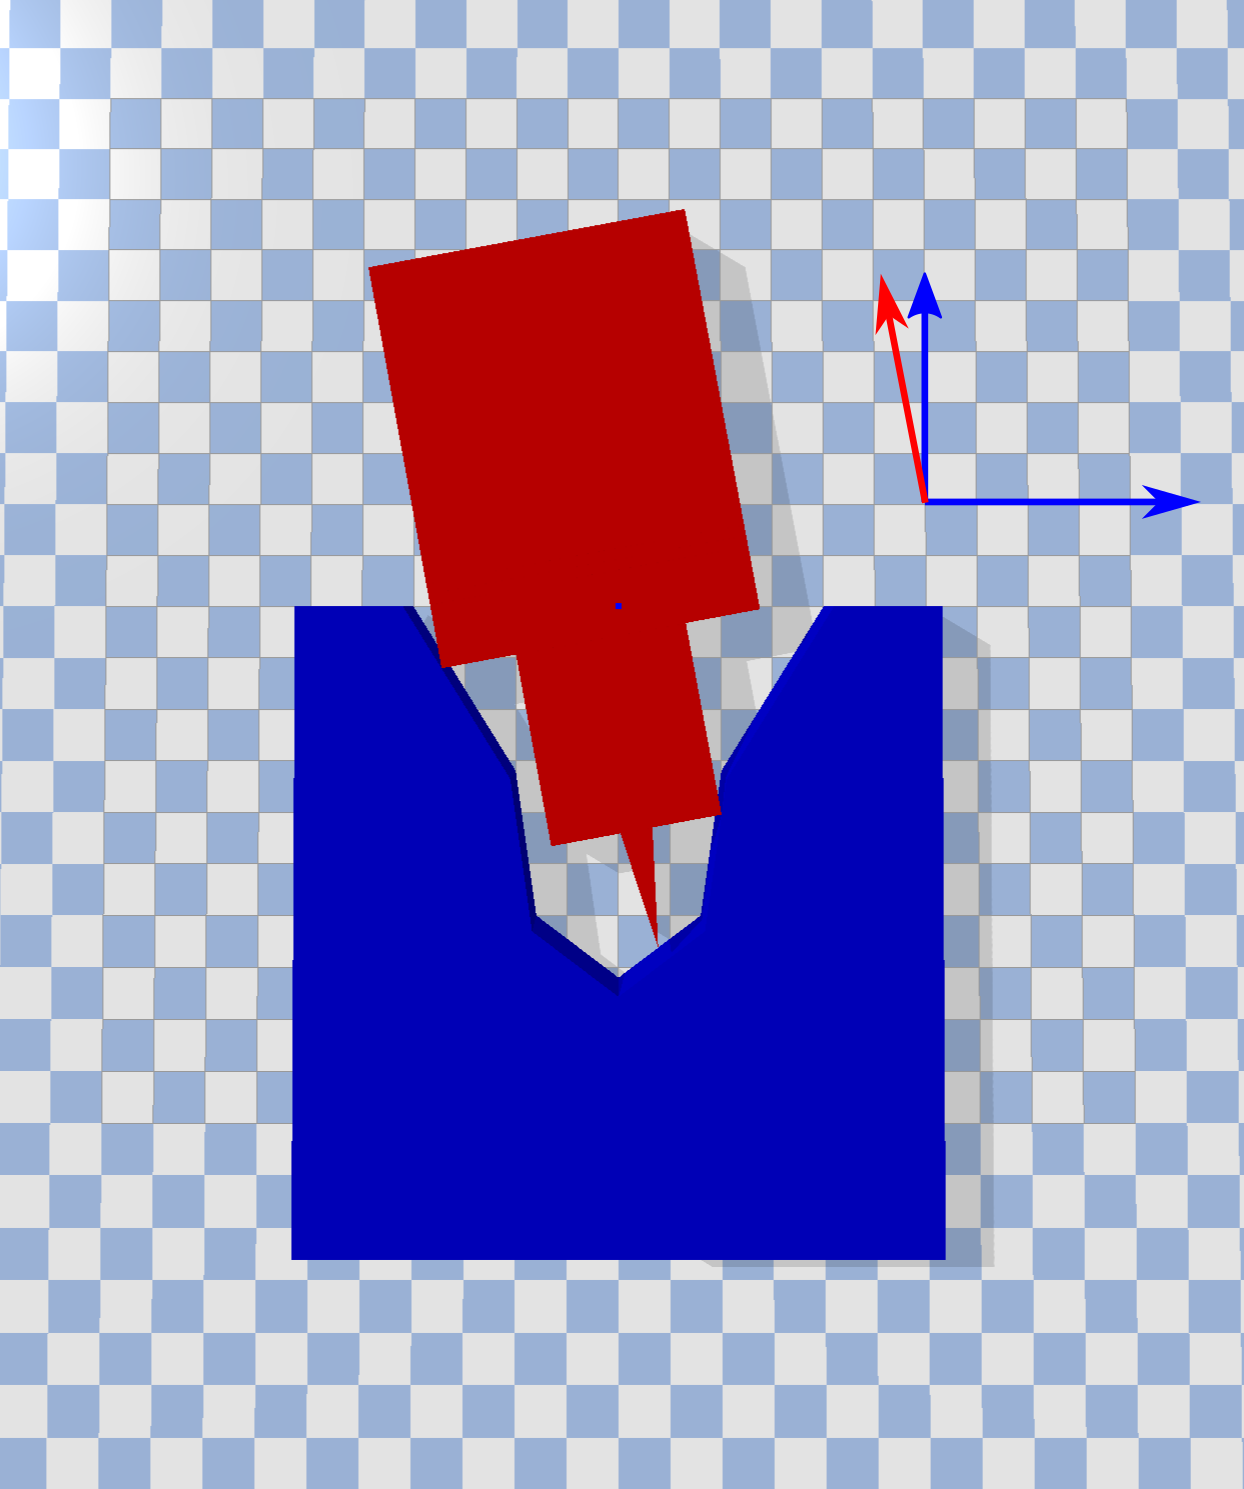
\includegraphics[height=1.2in]{figures/initial_max_rotate.png}
\end{center}
\caption{The maximum rotation after insertion for an arbitrary joint design. }
\label{fig:initial_max}
\end{subfigure}
\begin{subfigure}[t]{0.23\textwidth}
\begin{center}
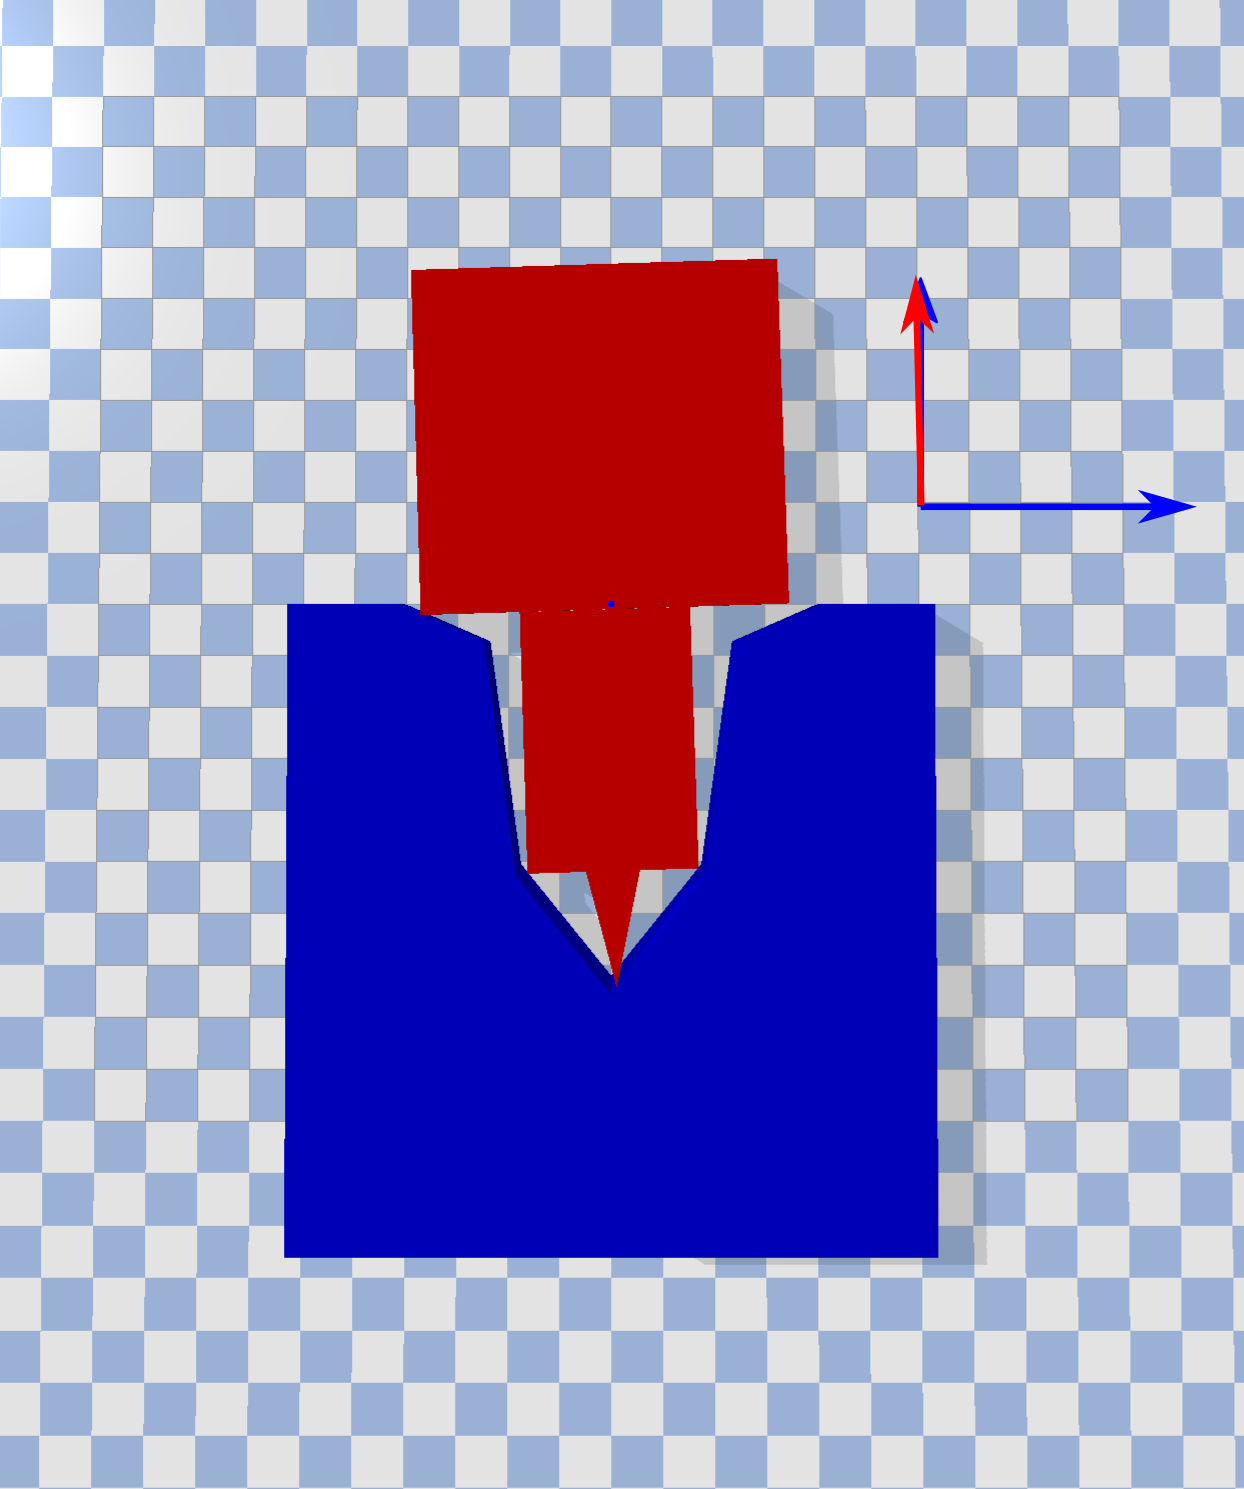
\includegraphics[height=1.2in]{figures/optimal_max_rotate.png}
\end{center}
\caption{The maximum rotation after insertion for an optimized joint design. }
\label{fig:optimal_max}
\end{subfigure}
\begin{subfigure}[t]{0.44\textwidth}
\begin{center}
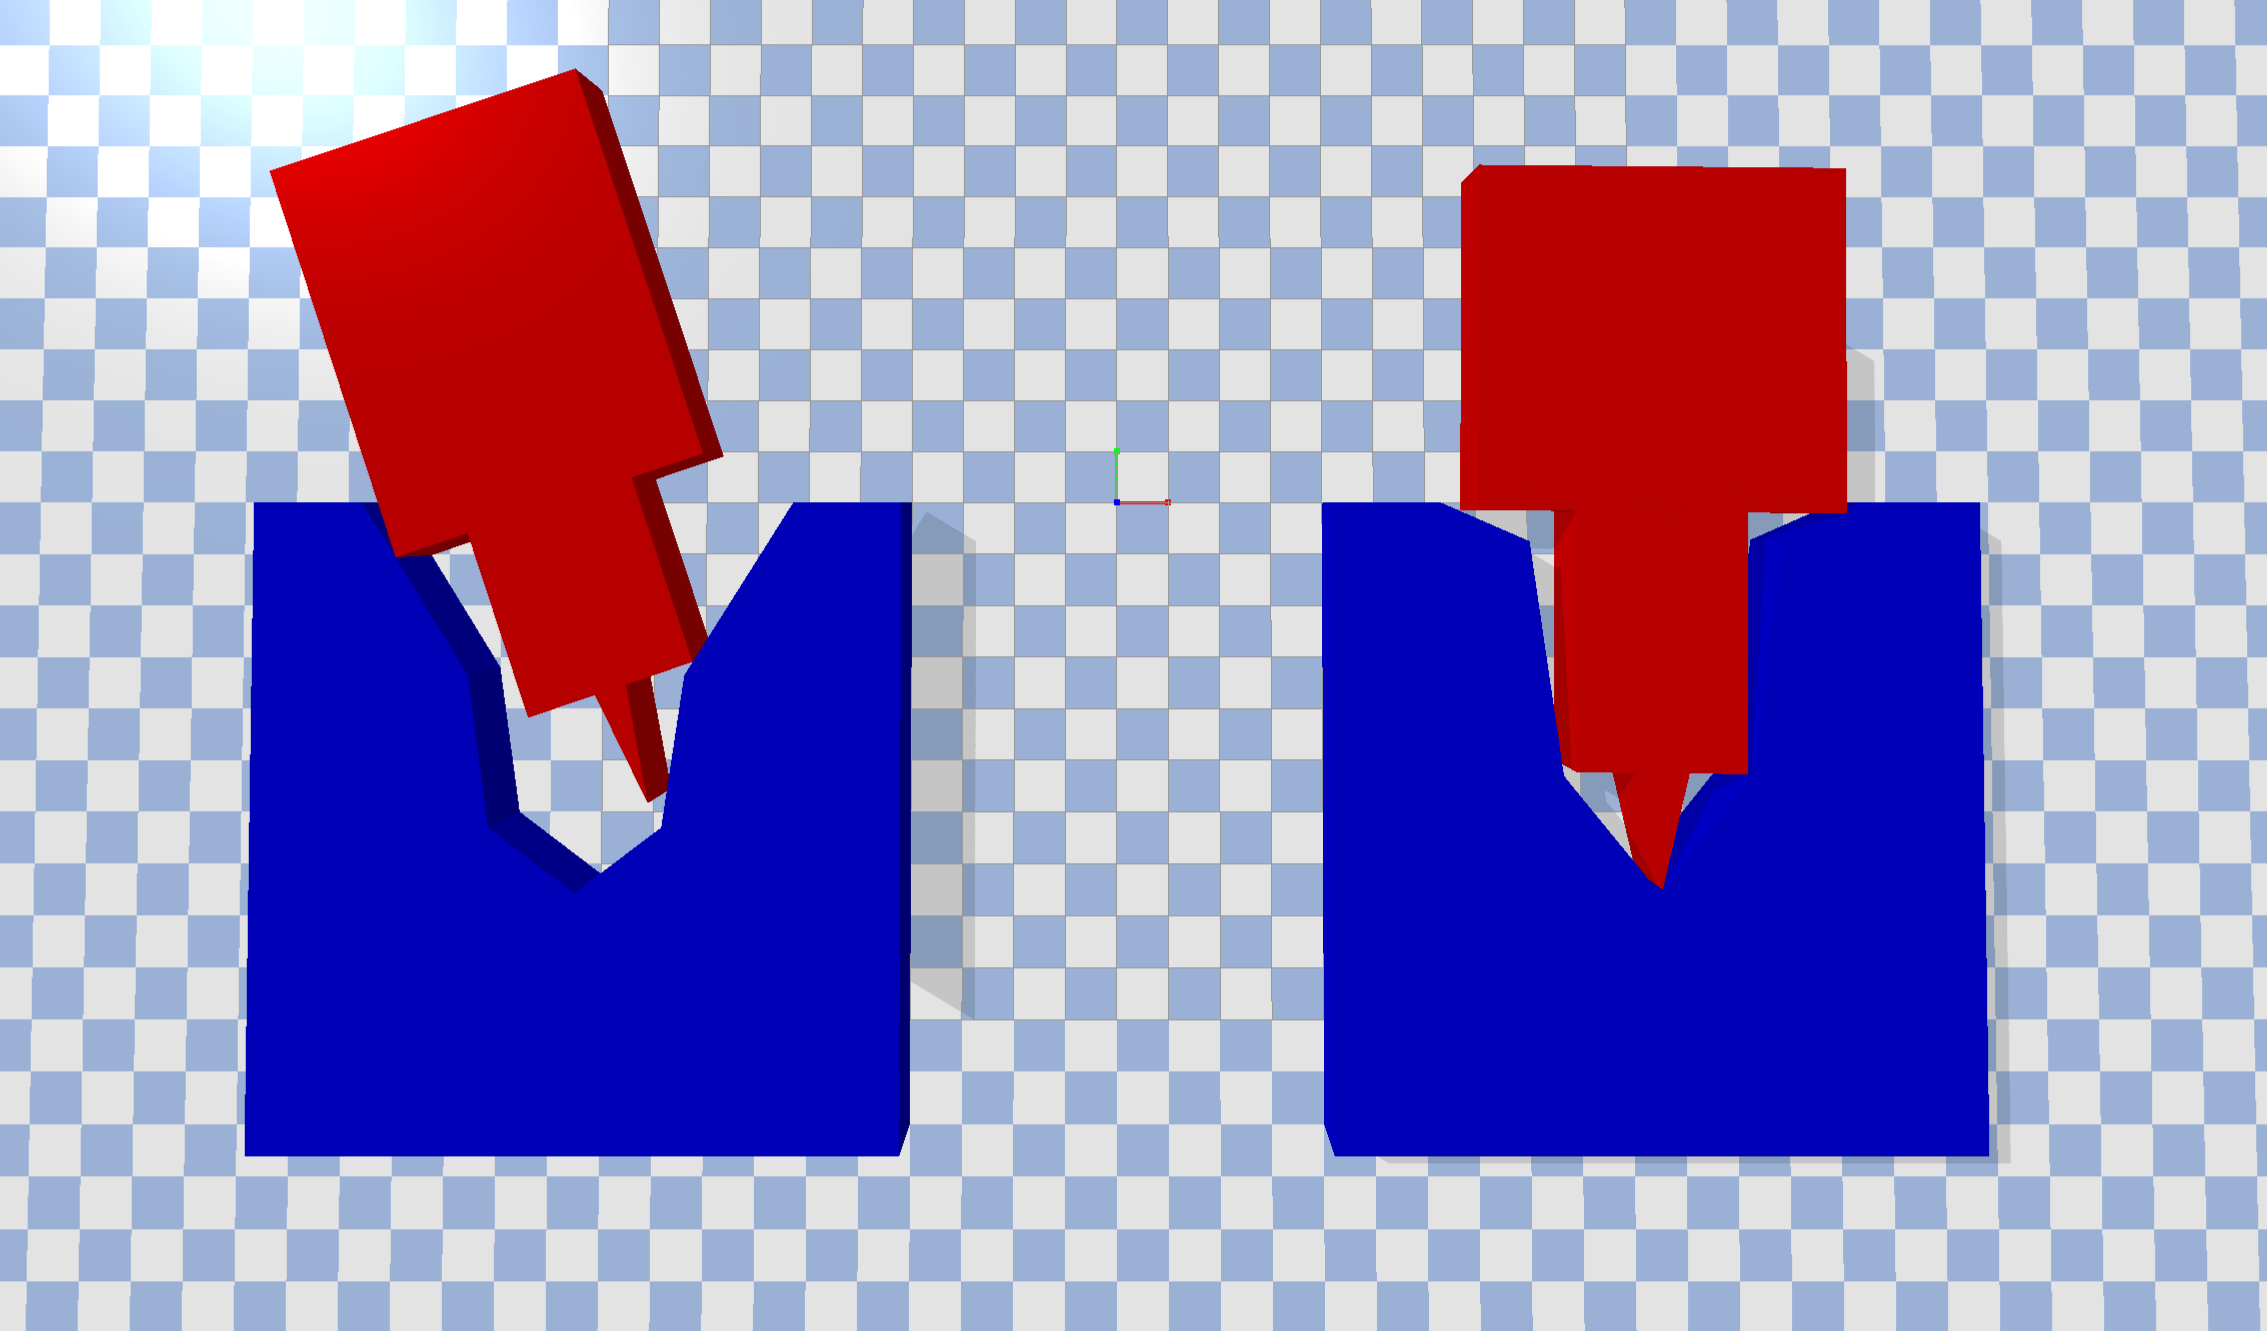
\includegraphics[height=1.2in]{figures/stuck.png}
\end{center}
\caption{During insertion, arbitrary design may get {\em stuck} before reaching the sink, while the optimized joint can reach the sink regardless of the initial condition. }
\label{fig:stuck}
\end{subfigure}
\caption{Simulation of insertion and stability after insertion in bullet physics engine. }
\label{fig:simulation}
\end{center}
\end{figure}

To verify the design process generated joints that are {\em better} according to our criteria, we used bullet physics engine~\cite{coumans2019} to simulate and compare the insertion with different designs. Compared to an arbitrary design with same $m$ and $n$, the optimized design (using the proposed process) shows much more stable behavior after insertion, when all designs can be successfully inserted into the socket, as shown in Figure~\ref{fig:initial_max} and~\ref{fig:optimal_max}. Using the optimized design, even when insertion starts from different initial configurations, all insertion simulations are successful. While with a joint design that presents undesired sinks, some simulations of insertion failed and {\em stuck} at the configuration corresponding to the undesired sinks, as shown in Figure~\ref{fig:stuck}. In the figures shown above, only part of the peg block is shown, as our analysis is based on the peg and socket relation along. The contact between blocks may affect the design process, which we did not consider in the derived joint designs. In the future work, we plan to include the contact between the blocks in the design process. 

\section{Conclusion and future work}

In this work, we present an automated design process that can find the {\em best} insertion-based joint design, guaranteeing the success of insertion and achieve the most stability after insertion. The analysis is done in 2D, and the design output can be projected into 3D for the actual block design. This work focus on the planar design process, while different projection approaches will be analyzed and compared in the future work. The design process takes the manufacturing error and execution error into account, and the design results are error tolerant. The results are validated using bullet physics engine, confirming our analysis and the quality of the design output. We found that in the planar case, socket with six edges and peg with five points can achieve the best stability after insertion, while guaranteeing the success of insertion. 


\renewcommand*{\bibfont}{\small}
\printbibliography

\end{document}
